\documentclass[a4paper]{article}

% 한글 환경 설정
\usepackage[finemath]{kotex}
\usepackage{dhucs-cmap}
\pdfmapfile{=unttf-pdftex-kotex.map}
\usepackage[verbose=true]{microtype}
\DeclareMicrotypeSet{dhucsmicro}{encoding=LUC}
\UseMicrotypeSet[expansion]{dhucsmicro}

% 기타 환경 설정
\usepackage{graphicx}
\usepackage{amsmath}
\usepackage{palatino}
\usepackage[onehalfspacing]{setspace}
\usepackage{url}
\usepackage{hyperref}
\usepackage[usenames,dvipsnames]{color}
\usepackage{multicol}

% Page Layout
\usepackage{calc}
\addtolength{\hoffset}{-50pt}
\addtolength{\voffset}{-10pt}
\addtolength{\marginparwidth}{-20pt}
\addtolength{\textwidth}{100pt}
\addtolength{\textheight}{25pt}
\addtolength{\skip\footins}{8pt}
\setlength{\columnsep}{20pt}
\setlength{\footnotesep}{4pt}

\begin{document}
\title{CS492 Distributed Systems \& Algorithms\\ \textit{Final Report:} \textbf{Mr.CL}}
\author{20030767 최종욱, 20050145 김준기, 20060080 김민국}
\date{2009년 12월 24일}
\vspace{-40pt}
\maketitle

\begin{multicols}{2}
\section{Introduction}
Matrix multiplication은 과학 연산과 데이터 마이닝 등 여러 분야에서 많이 이용되는 기본적인 연산이며 매우 방대한 크기의 matrix를 이용해 계산하는 경우가 자주 발생한다.
그래서 이를 최적화 시키기 위한 많은 시도가 이루어져 왔는데, 우리는 MapReduce를 통해서 임의의 대용량 matrix를 가지고 multiplication을 수행하는 알고리즘을 개발하고자 하였다.

이 과정에서 이렇게 방대한 크기의 matrix를 다룰 수 있게 하는 것도 중요하지만, 연산 시간을 줄이는 노력 또한 함께 이루어져야 한다.
따라서 더 빠르게 계산을 수행할 수 있도록 matrix multiplication 과정에서 GPU에 의한 가속 기능을 도입하였다.
GPU는 그 성격상 실수와 matrix 연산에 특화되어 일반 CPU보다 훨씬 더 나은 성능을 보여주기 때문이다.

이러한 아이디어를 바탕으로 우리는 GPU를 설치한 클러스터 위에서 동작하는 Hadoop MapReduce를 이용한 matrix multiplication 알고리즘을 설계하고 이의 성능을 측정해보았다.
이를 통해 분산 시스템을 이용한 대용량의 데이터에 대한 확장성(scalability)을 얻고, GPU로 연산 속도를 향상시킴으로써 이전보다 개선된 matrix multiplication을 수행할 수 있었다.

\section{Design Overview}
\subsection{Assumptions}chart-java-vs-jcublas
우리가 목표로 하는 시스템의 효과적인 설계와 구현을 위해 약간의 가정이 필요하다.
\begin{itemize}
	\item Matrix의 각 원소들은 single precision floating point format을 통해서 표현된다. CUDA 라이브러리에서 double precision을 지원하기는 하지만 JCublas와 연동할 때 내부적인 변환에 따른 성능 저하 및 심각한 계산 오류가 발생해 사용할 수 없었다.\footnote{파일럿 테스트 과정에서 각 원소가 $[0,1]$ 구간에서 무작위로 생성된 $100 \times 100$ 행렬 2개을 곱했을 때 single precision으로 입력을 주어 계산하면 한 원소가 250 정도의 값을 가지는데 double precision 입력의 경우 0에 매우 가까운 실수가 되어 correctness 판정을 통과하지 못했다.}
	\item 각 matrix는 dense matrix이다. Sparse matrix의 경우 모든 원소를 연속적으로 저장하지 않고 개별적인 쌍으로 저장하기 때문에 원소를 접근할 때 index를 key로 하는 탐색 작업이 필요하다. 이것은 GPU처럼 연속적인 메모리를 할당하여 한꺼번에 pipelining하는 구조에 적합하지 않으므로 우리는 dense matrix인 경우만 고려하였다.
	\item 작은 클러스터에서 HDFS 상의 임의의 파일을 읽어올 때 걸리는 시간은 평균적으로 동일하다. 이는 구현을 간단히 하기 위해 Hadoop이 제공하는 data locality를 고려하지 않는다는 뜻이다.
\end{itemize}

\subsection{Block Approach}
Dense matrix multiplication을 수행할 때 I/O 병목에 의해 계산 속도가 제약되는 이유는 $O(n^3)$ 번의 곱셈 횟수와 $O(n^2)$ 개의 원소를 불러오는 횟수가 matrix가 커질수록 큰 차이가 나기 때문이다.
특히 이러한 I/O 병목 문제는 multi-processor나 네트워크 기반 클러스터로 규모를 확대할수록 더욱 심각해지는데, 이는 프로세서끼리 혹은 클러스터 상의 컴퓨터끼리의 통신 대역폭이 제한되어 있기 때문이다.
따라서 우리는 프로세서의 성능을 최대한으로 활용하기 위해 프로세서가 처리할 데이터가 가능한 한 지속적으로 공급될 수 있도록, 혹은 데이터를 한 번 불러왔을 때 가능한 한 많이 반복적으로 연산에 활용하도록 알고리즘과 코드를 작성해야 한다.

이 문제를 해결하기 위해 우리는 matrix를 block 단위로 쪼개어 적절히 이를 분산시켜 multiplication을 수행하는 방법을 선택하였다.
만약 각 block들이 적당히 큰 상황이라면, 우리는 각 노드 상에서 이러한 block들의 각 element들을 한 번 불러와 적당한 횟수만큼 multiplication에 다시 이용할 수 있을 것이다.
이때 각 block들은 일반적으로 square matrix지만 아닌 경우도 있을 수 있으므로 알고리즘에 따라서 적절한 block decomposition을 구현하는 것이 중요하다.

\subsubsection{Outer Product Algorthm}
Matrix multiplication을 구현하는 방법으로는 정의대로 계산하는 $O(n^3)$ 짜리와 $O(n^{2.376})$의 시간이 걸리는 Coppersmith-Winograd 알고리즘 등이 있으나, 우리는 MapReduce에서 쓰기 알맞게 outer product를 응용한 방식을 사용하였다.

\begin{align} \label{eq:OuterProduct}
&\begin{bmatrix} \color{Red}1 & \color{Green}2 & \color{NavyBlue}3 \\ \color{Red}4 & \color{Green}5 & \color{NavyBlue}6 \\ \color{Red}7 & \color{Green}8 & \color{NavyBlue}9 \end{bmatrix} \begin{bmatrix} \color{Red}a & \color{Red}d \\ \color{Green}b & \color{Green}e \\ \color{NavyBlue}c & \color{NavyBlue}f \end{bmatrix} \\ \nonumber
&=\begin{bmatrix} \color{Red}1a & \color{Red}1d \\ \color{Red}4a & \color{Red}4d \\ \color{Red}7a & \color{Red}7d \end{bmatrix} + \begin{bmatrix} \color{Green}2b & \color{Green}2e \\ \color{Green}5b & \color{Green}5e \\ \color{Green}8b & \color{Green}8e \end{bmatrix} + \begin{bmatrix} \color{NavyBlue}3c & \color{NavyBlue}3f \\ \color{NavyBlue}6c & \color{NavyBlue}6f \\ \color{NavyBlue}9c & \color{NavyBlue}9f \end{bmatrix}
\end{align}

Eq.~\eqref{eq:OuterProduct}를 보면 두 matrix의 열과 행 vector들을 각각 outer product를 취하여 나온 matrix들을 모두 더하면 전체 multiplication 결과를 완성할 수 있음을 알 수 있다.

여기서 각 원소들은 하나의 실수가 아니라 submatrix(앞에서 block이라고 표현했던 matrix의 일부)여도 되므로, 우리는 이처럼 block 단위로 쪼개고 다시 합치는 과정을 MapReduce로, 각 block들을 곱하는 과정을 개별 노드에서 GPU로 가속하는 방식을 취하였다.
이렇게 하면 $O(n^3)$ 만큼의 연산 시간이 걸리지만, block 단위로 분산 저장되어 있을 경우 I/O 비용을 크게 줄일 수 있다는 장점이 생긴다.

\subsection{NVIDIA CUDA}
실험에 사용된 클러스터 상의 모든 노드에는 NVIDIA의 그래픽 카드가 장착되어 있다.
NVIDIA에서는 CUDA라는 기술을 통해 개발자들이 C 언어로 직접 GPU에서 동작하는 프로그램을 만들 수 있도록 하고 있다.
이것을 기반으로 BLAS API\footnote{Basic Linear Algebra Subprograms. Vector-Vector, Vector-Matrix, Matrix-Matrix 연산들을 단계별로 정의하고 있다.}를 구현한 CUBLAS를 이용하면 matrix multiplication을 GPU를 이용하여 수행할 수 있다.


\section{Implementation}
\subsection{Cluster Setup}
학과나 NexR에서 제공하는 클러스터는 가상화 기술을 기반으로 하고 있어 GPU 활용이 불가능하였기 때문에 개인용 PC 2개를 아래와 같이 구성하였다.
\begin{itemize}
	\item Intel Core2 Q9400 (2.66GHz), RAM 4GB, SATA2 HDD 640GB, NVIDIA GTX250
	\item Intel Core2 E6600 (2.4GHz), RAM 4GB, SATA2 HDD 320GB, NVIDIA GTX250
	\item Network: 100Mbps Ethernet (ipTIME Pro54G 공유기로 private network 구성)
\end{itemize}

\subsection{Data Model}
모든 matrix는 HDFS에 저장된다. $N \times N$ 크기를 가지는 2개의 matrix는 임의로 붙인 이름에 따라 디렉토리가 만들어지고 그 아래에 block 별로 다시 디렉토리가 만들어져 분할 저장된다.
예를 들어 example이라는 이름의 matrix의 위에서 5번째(행), 왼쪽에서 3번째(열) 위치에 있는 block은 \texttt{/example/5/3} 디렉토리에 실제 원소들의 값이 저장되는 것이다.
이렇게 저장된 데이터는 MapReduce 실행 과정에서 필요에 따라 꺼내와 사용하게 되며, 이때 이 데이터들은 Hadoop MapReduce의 입출력 메카니즘을 이용하지 않고 직접 파일시스템 API를 통해 HDFS로 접근하기 때문에 data locality는 고려되지 않았다.

\subsection{MapReduce Execution}
\subsubsection{Mapper}
\begin{description}
	\item[Input] \hfill \\
	$(\text{key}, \text{value})  = (l, (A, B, r))$ ($l$은 텍스트 입력의 문자 번호로 무시됨)
	\begin{itemize}
		\item $A$ : 행렬 $\mathbf{A}$의 이름
		\item $B$ : 행렬 $\mathbf{B}$의 이름
		\item $r$ : 곱셈을 수행할 $\mathbf{B}$의 block들의 행과 $\mathbf{A}$의 block들의 열을 의미한다. 즉, block 단위로 바라보았을 때 행렬 $\mathbf{A}$의 $r$열과 행렬 $\mathbf{B}$의 $r$행을 곱한다.
	\end{itemize}
	\item[Output] \hfill \\
	$(\text{key}, \text{values}) = ((A, B), C_r)$
	\begin{itemize}
		\item $A$, $B$ : 입력과 같다.
		\item $C_r$ : 연산의 결과로 HDFS 상의 \texttt{\_\_tmp/A\_B\_r} 디렉토리에 위 곱셈의 결과인 $N \times N$ matrix $\mathbf{C}_r$이 저장되는데 그 위치를 가리킨다.
	\end{itemize}
	\item[Mechanism] \hfill \\
	곱셈을 수행하고자 하는 block의 행과 열 번호를 알고 있으므로 우리는 다음과 같이 계산할 수 있다. $m$은 $\mathbf{A}$의 block 열 개수이고 $\mathbf{A}(i,j)$가 행렬 $\mathbf{A}$를 block 단위로 보았을 때 $i$행 $j$열 block이라고 하고 결과값을 가지는 행렬을 $\mathbf{C}_r$라 하면,
	\begin{equation*}
		\mathbf{C}_r(i,j) = \mathbf{A}(i,r) \times \mathbf{B}(r,j) \:\:\forall \,i,j=1..m
	\end{equation*}
	가 성립한다. 따라서 $m \times m$개의 block으로 이루어진 $N \times N$ 행렬 $\mathbf{C}_r$를 구할 수 있으며 이를 저장한다.
	이 곱셈 과정이 JCublas로 가속된다.
\end{description}
\subsubsection{Reducer}
\begin{description}
	\item[Input] \hfill \\
	$(\text{key}, \text{values}) = ((A, B), C_r)$
	\begin{itemize}
		\item $A$, $B$, $C_r$ : Mapper의 출력과 같다.
	\end{itemize}
	\item[Output] \hfill \\
	$(\text{key}, \text{value}) = ((A, B), C)$
	\begin{itemize}
		\item $A$, $B$ : Mapper의 출력과 같다. 
		\item $C$ : 최종 결과 matrix $\mathbf{C}$가 저장된 위치를 가리킨다.
	\end{itemize}
	\item[Mechanism] \hfill \\
	Mapper에서 만든 $\mathbf{C}_r$들을 모두 더하여 최종 곱셈 결과 matrix $\mathbf{C}$를 생성한다.
	Reducer의 일은 Combiner에서도 동일하게 수행하여 전체 계산이 좀더 빠르게 수행되도록 하였다.
\end{description}

\section{Performance Analysis}
\subsection{Pure Java vs. JCublas}
\begin{minipage}{\linewidth}
	\centering
	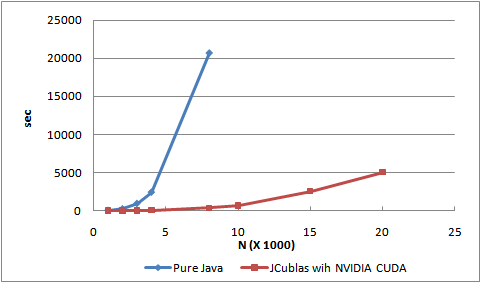
\includegraphics[width=0.9\linewidth]{chart-java-vs-jcublas.png}
	\figcaption{Matrix size에 따른 방식별 연산 수행시간 비교}
	\label{fig:java-vs-jcublas}
\end{minipage}
\subsection{Variable block size with Java}
\begin{minipage}{\linewidth}
	\centering
	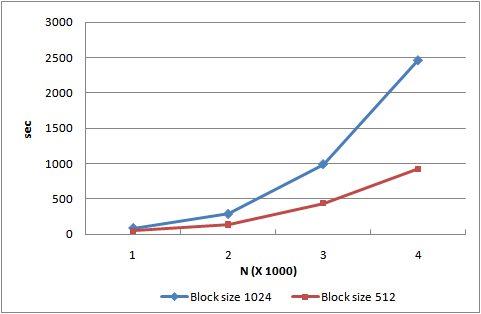
\includegraphics[width=0.9\linewidth]{chart-java-with-variable-block-size.png}
	\figcaption{Java에서 block size 별 연산 수행시간 비교}
	\label{fig:java-blocksize}
\end{minipage}
\subsection{Variable block size with JCublas}
\begin{minipage}{\linewidth}
	\centering
	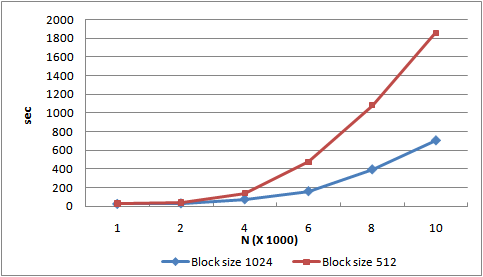
\includegraphics[width=0.9\linewidth]{chart-jcublas-with-variable-block-size.png}
	\figcaption{JCublas에서 block size 별 연산 수행시간 비교}
	\label{fig:jcublas-blocksize}
\end{minipage}

\section{Related Works: Hama}
프로젝트 초기에는 matrix multiplication 구현 자체에 대한 부담을 줄이고 GPU를 이용한 가속에 집중하기 위해 이미 Hadoop 기반으로 다양한 matrix 연산을 구현한 Apache 재단의 Hama 프로젝트를 이용하였다.
특히 Hama는 dense matrix 곱셈을 block 방식으로 구현하고 있었다.
하지만 다음과 같은 이유로 Hama 프로젝트를 사용하지 않고 직접 Hadoop MapReduce로 구현하게 되었다.
\begin{itemize}
	\item Hama가 Hadoop 기반 데이터베이스인 HBase를 이용하고 있었고, 아직 HBase가 성능 측면이나 프로젝트 자체의 성숙도가 떨어져 실제 우리가 원하는 규모의 연산을 돌리기에는 적합치 않았다.\footnote{우리 목표는 $10^4$이나 $10^5$ 정도인데, Hama 개발자 스스로 자신의 블로그에서 $5000 \times 5000$ 정도가 한계라고 밝히고 있음.\\\url{http://blog.udanax.org/2009/01/distributed-matrix-multiplication-with.html}}
	HBase를 들어내려면 Hama를 거의 처음부터 다시 짜야 한다.
	\item Hama에서는 matrix의 원소들을 기본으로 double precision으로 처리하고 있는데 여기에 CUDA를 연동시키려면 single precision으로 변환하는 과정이 필요하여 불필요한 성능 저하를 발생시키고 이렇게 동작하도록 Hama의 코드 전체를 바꾸는 것이 용이하지 않았다.
	\item 곱셈 과정에서 block 쌍들을 모두 별도로 저장하였다가 불러오는데, 이 과정의 I/O complexity가 $O(n^3)$이어서 새로운 접근 방법이 필요했고 결국 이것이 $O(n^2)$으로 줄어든 outer product algorithm을 새로 구현해야 했다.
\end{itemize}

\section{Conclusion}
{\color{BurntOrange} TODO: 실험 결과 정리}
이번 실험에서 빠진 부분이 같은 크기의 matrix를 처리할 때 클러스터의 노드 수가 늘어나면 얼마나 성능 향상 효과가 있는가 하는 점으로, scalability를 확보하고자 MapReudce를 도입한 의미를 살리려면 향후 반드시 조사해야 할 부분이다.

이번 실험의 경우 GPU가 장착된 클러스터를 대규모로 구축할 수 없었고 실제 하드웨어 환경을 구축하기까지 많은 시간이 걸렸다는 점이 걸림돌로 작용하였다.
또한 CUDA에 대한 사용 경험이 없었기 때문에 드라이버 설치나 이용 과정에서도 시행착오를 겪어야 했고, Hama의 한계나 JCublas의 double precision 지원 문제 등도 이에 일조하였다.
하지만 이렇게 기존의 연산 문제를 다른 각도에서 풀어봄으로써 확실히 MapReduce의 가능성과 한계를 알 수 있었다는 점은 흥미롭다.

앞으로 더 해보고 싶은 것은 이번에 활용하지 못한 Hadoop의 data locality 이점을 살릴 수 있도록 구현 코드의 구조를 다시 한 번 손보고, CUDA를 이용하지 않고 CPU로만 계산하되 Java가 아닌 C로 최적화되어 작성된 CBLAS 라이브러리를 Java와 붙여서 GPU가 없는 환경에서도 어느 정도 성능 향상을 볼 수 있도록 하여 보다 범용적으로 쓰일 수 있게 하는 것이다.
또한 이 결과를 오픈소스로 잘 정리하여 누구나 활용 가능하도록 하였으면 한다.\footnote{현재 Google Code에 Mr.CL 프로젝트를 개설해둔 상태이다. \url{http://code.google.com/p/mrcl/} 참조.}

\end{multicols}
\end{document}
